\documentclass[12pt]{longnotes}
\usepackage{tlegacy} 
\usepackage{thranges}
\usepackage{silence}
\WarningFilter{latex}{Reference}
\graphicspath{{../../img/}}

\begin{document}
\paragraph{Числовые ряды и примеры оных}
\begin{defn}\label{defn:numseries}
  Пусть $(a_n)_{n=1}^\infty,\; a_n \in \R$~--- числовая последовательность.
  Тогда рядом можно назвать последовательность и желание её просуммировать\smiley.
  \begin{itemize}
    \item Элементы последовательности $(a_n)$~--- члены ряда.
    \item $S_n = \dsum_{k=1}^m a_k $~--- частичная сумма последовательности $(a_n)$
    \item $r_m = \dsum_{k=m+1}^\infty a_k$~---  остаток ряда.
    \item $S = \dsum_{k=1}^\infty a_k := \lim_{n \to \infty} S_n$~--- сумма ряда.
  \end{itemize} 
  В принципе, ряд можно попробовать формализовать как упорядоченную пару $\big((a_n),(S_n)\big)$.
  Или просто называть рядом некий цельный символ $\sum_{n=1}^\infty a_n$.
\end{defn}

\begin{defn}\label{defn:num}
  Ряд называется \emph{сходящимся} когда предел частичных сумм существует и конечен и 
  \emph{расходящимся} во всех остальных случаях.
\end{defn}

\begin{exmp}
  \[
    \sum_{k=1}^{\infty} \frac{1}{k(k+1)} = \frac{1}{1\cdot2} + \frac{1}{2\cdot3} + \frac{1}{3\cdot4} +\dotsb
  \]
  Посмотрим на член ряда:
  \[
    \frac{1}{k(k+1)} = \frac{1}{k} - \frac{1}{k+1}
  \]
  Перепишем ряд:
  \[
    \sum_{k=1}^{n} = \left( 1 - \frac{1}{2} \right) + \left( \frac{1}{2} - \frac{1}{3} \right) + \dotsb 
    + \left( \frac{1}{n} - \frac{1}{n+1} \right) = 1 - \frac{1}{n+1}
  \]
  Оно магически свернулось. Теперь: 
  \[
    S = \lim_{n\to \infty} \left( 1 - \frac{1}{n+1} \right) = 1
  \]
\end{exmp}
\begin{exmp}\label{exmp:geomseries}
  \[
    \begin{cases}
      \dsum_{n=0}^\infty q^n = \frac{1}{1-n}, & |q| < 1 \\
      \text{ ряд расходится },  & |q| \geqslant 1 \\
    \end{cases}
  \]
\end{exmp}

\paragraph{Общие свойства числовых рядов}
\begin{enumerate}
  \item $\dsum_{k=1}^\infty a_k \conv \Rightarrow a_k \xrightarrow[k\to \infty]{} 0$
  \item ряд сходится $\Leftrightarrow$ его остаток сходится.
  \item $\dsum_{k=1}^\infty(a_k + b_k) = \dsum_{k=1}^\infty a_k + \dsum_{k=1}^\infty b_k $
     (если любые  2 ряда сходятся, то сходится и третий).
   \item $\forall c\in \R\; \dsum_{k=1}^\infty c\,a_k = c \dsum_{k=1}^\infty a_k$
     (характер сходимости у рядов одинаковый)
   \item $\dsum_{k=1}^\infty a_k \conv 
     \Leftrightarrow r_m \! = \!\!\dsum_{k=m+1}^\infty a_k \xrightarrow[m\to\infty]{} 0$
\end{enumerate}
\begin{stat}[Критерий сходимости Больцано-Коши]\label{stat:bkseriesconv}
  \[
    \sum_{k=1}^\infty a_k \conv \Leftrightarrow \forall\,\varepsilon > 0 \; \exists\, N: \forall\, n > N
    \; \forall\, p > 0 \;\: \left| \sum_{k=n+1}^{n+p} a_k \right| < \varepsilon
  \]
\end{stat}

\paragraph{Положительные ряды. Признаки сравнения}
\begin{defn}
  Ряд положителен, если $\forall k \; a_k \geqslant 0$
\end{defn}

\setcounter{thrm}{-1}
\begin{stat}
  Всегда $\exists\, S\in [0; +\infty]$
\end{stat}

\begin{stat}[Первый признак сравнения]\label{stat:cmpseries1}
  Пусть $\forall\, n \; a_n \geqslant b_n \geqslant 0$. Тогда
  \begin{align*}
    \sum_{k=1}^{\infty} a_k \conv   &\Rightarrow \sum_{k=1}^{\infty} b_k \conv \\ 
    \sum_{k=1}^{\infty} a_k \noconv &\Leftarrow \sum_{k=1}^{\infty} b_k \noconv \\ 
  \end{align*}
\end{stat}
\begin{rem*}
 Хватит выполнения неравенства в $V(\infty)$, всё равно сходимость определяют только остатки.
\end{rem*}
\begin{stat}[Второй признак сравнения]\label{stat:cmpseries2}
  Пусть $\forall\, n \; a_n \geqslant 0, b_n > 0$ и также
  \[
    \exists\, \lim_{n\to \infty}\frac{a_n}{b_n} = L \in [0; +\infty]
  \]
  Тогда: 
  \begin{align*}
    L <+\infty \Rightarrow \left( \sum_{k=1}^{\infty} b_k \conv \Rightarrow \sum_{k=1}^{\infty} a_k \conv \right)\\
    L > 0 \Rightarrow \left( \sum_{k=1}^{\infty} a_k \conv \Rightarrow \sum_{k=1}^{\infty} b_k \conv \right)\\
  \end{align*}
\end{stat}

\begin{imp}
  При $0 < L < +\infty$ ряды ведут себя одинаково
\end{imp}

\parrange{2}{Признаки Даламбера и Коши}

\begin{thrm}[Признак Даламбера]\label{thrm:dalambconv}
  Пусть $\sum a_n$~--- положительный ряд и 
  \[
    \exists\, D = \lim_{n\to\infty} \frac{a_{n+1}}{a_n}, \; D \in [0;+\infty]
  \]
  Тогда 
  \begin{enumerate}
    \item $D < 1$ $\Rightarrow$ ряд сходится
    \item $D > 1$ $\Rightarrow$ ряд расходится
    \item $D = 1$ $\Rightarrow$ непонятно
  \end{enumerate}
\end{thrm}
\begin{thrm}[Признак Коши]\label{thrm:cauchyconv}
  Пусть $\sum a_n$~--- положительный ряд и 
  \[
    \exists\, C = \lim_{n\to\infty} \sqrt[n]{a_n}, \; C \in [0;+\infty]
  \]
  Тогда 
  \begin{enumerate}
    \item $C < 1$ $\Rightarrow$ ряд сходится
    \item $C > 1$ $\Rightarrow$ ряд расходится
    \item $C = 1$ $\Rightarrow$ непонятно
  \end{enumerate}
\end{thrm}

\begin{rem}
  Оба признака: и Коши и Даламбера~--- основаны на сравнении ряда с геометрической прогресиией~\ref{exmp:geomseries}.
  А сумма геометрической прогрессии сходится, когда её знаменатель $ < 1$. А $q=1$~--- точка в которой
  формула суммы геометрической прогресии не существует. Так что она особенная $\smiley$.
\end{rem}

\begin{rem}
  В качестве примера к 3 пункту обеих теорем годится ряды $\sum \frac{1}{n}$ и $\sum \frac{1}{n^2}$.
  Второй сходится, а первый~--- нет.
\end{rem}

\parrange{2}{Верхний и нижний пределы последовательности}
\begin{defn}\label{defn:limsup}
  Пусть $(x_n)$~--- целочисленная последовательность. Тогда 
  \begin{align*}
    & \underline{\ell} = \llim_{k\to \infty} x_k := \lim_{n\to \infty} \inf_{k\geqslant n} x_k \\
    & \overline{\ell} = \uplim_{k\to \infty} x_k := \lim_{n\to \infty} \sup_{k\geqslant n} x_k
  \end{align*}
  где $\overline{\ell}, \underline{\ell}$~--- верхний и нижний пределы соответственно.
\end{defn}
\begin{rem}
  Можно ещё конечно отдельно упомянуть про случаи с $\pm \infty$, но вроде как все они уже заложены
  в определение предела.
\end{rem}
\begin{rem}
  Верхний и нижний пределы существуют, так как последовательность супремумов/инфимумов монотонна.
\end{rem}

\begin{defn}
  Пусть $(x_n)$~--- целочисленная последовательность, $(x_{n_k})$~--- её подпоследовательность. 
  Тогда $c\in \overline{\R}$:
  \[
    c = \lim_{k\to \infty} x_{n_k} 
  \]
  называется частичным пределом последовательности.
\end{defn}

\begin{thrm}[Теорема о трёх пределах?]
  \[
    \exists\, \lim_{n\to\infty} x_n 
    \Leftrightarrow \llim_{n\to\infty} x_n = \uplim_{n\to\infty} x_n = \lim_{n\to\infty} x_n
  \]
\end{thrm}
\begin{ittproof}
  Следствие теоремы~\ref{thrm:partlimset}
\end{ittproof}

\begin{thrm}[о множестве частичных пределов]\label{thrm:partlimset}
  Пусть $(x_n)$~--- целочисленная последовательность, $\overline{\ell}, \underline{\ell}$~--- её 
  верхний и нижний пределы соответственно. 
  \begin{enumerate}
    \item $c$~--- частичный предел $\Rightarrow \underline{\ell} \leqslant c \leqslant \overline{\ell}$
    \item $\underline{\ell}, \overline{\ell}$ сами являются частичными пределами
  \end{enumerate}
\end{thrm}

\begin{ittproof}
  Пусть 
  \[
    \overline{x_n} = \sup_{i\geqslant n} x_i,\;\underline{x_n} = \inf_{i\geqslant n} x_i,\;
    c = \lim_{k\to \infty} x_{n_k}. 
  \]
  \begin{enumerate}
    \item Из определения $\overline{x_n}$, $\underline{x_n}$ и правила 3 полицейских: 
      \[
        \underline{x_{n_k}} \leqslant x_{n_k} \leqslant \overline{x_{n_k}} \xrightarrow[k\to \infty]{}
        \underline{\ell } \leqslant c \leqslant \overline{\ell}
      \]
      ( тут они ещё не подспоследовательности, но вот брать $n_k$ элемент мы уже умеем ).
    \item Докажем условие для $\overline{\ell}$, для инфимумов там то же самое будет. Из определения предела
      \[
        \forall\, V_1(\overline{\ell}) \;\:\exists\, N \colon \forall n > N \;\: \overline{x_n} \in V_1 
      \]
      К тому же
      \[
        \forall\, n, V_2(\overline{x_n}) \;\: \exists\, k > n \colon x_k \in V_2^- \subset V_2 \text{ 
          ( иначе $\overline{x_n}$ не супремум $\{x_k \mid k\geqslant n\}$). }
      \]
      Тогда $x_k \in V_1 \cup V_2$. А такими объединениями можно собрать любую окрестность.
  \end{enumerate}
\end{ittproof}

\paragraph{Обобщённый признак Коши}
\begin{thrm}\label{thrm:enhcauchyconv}
  Пусть $\sum a_n$~--- положительный ряд и 
  \[
    C = \uplim_{n\to\infty} \sqrt[n]{a_n}, \; C \in [0;+\infty]
  \]
  Тогда 
  \begin{enumerate}
    \item $C < 1$ $\Rightarrow$ ряд сходится
    \item $C > 1$ $\Rightarrow$ ряд расходится
    \item $C = 1$ $\Rightarrow$ непонятно
  \end{enumerate}
\end{thrm}
\begin{rem}
  В отличие от ``обычного'' признака Коши~\ref{thrm:cauchyconv}  тут не стоит вопрос о существовании предела,
  он есть всегда. Этим усиленный признак и лучше.
\end{rem}

\paragraph{Интегральный признак сходимости ряда}
\begin{thrm}
  Пусть $f\in C\big([1;+\infty)\big)$, $f\geqslant 0 $, $f \searrow [1;+\infty)$. 
    Пусть также $a_n  = f(n)$, $n\in \N$.
  Тогда 
  \[
    \sum_{n=1}^{\infty} a_n \conv \Leftrightarrow \int_{1}^{\infty} f \conv
  \]
\end{thrm}

\begin{ittproof}
  Пусть $F(t) = \int_1^t f$, тогда $F \nearrow [1;+\infty)$, $A_n \nearrow$. Значит, все пределы существуют.
    На основании этого немного перепишем условия:
  \begin{align*}
    \int_1^\infty f \conv &\Leftrightarrow \exists\,\sup\limits_{t\geqslant1} F(t) \in \R \\
    \sum_{k=1}^\infty a_k \conv &\Leftrightarrow \exists\,\sup\limits_{n\in\N} A_n \in \R 
  \end{align*}
  \begin{description}
    \item[\circlearound{$\Leftarrow$}] Пусть $k\in \N $, $k \leqslant x \leqslant k+1$. Тогда из
      убывания $f$
    \[
      \int_{k}^{k+1} f(x)\, dx \geqslant \int_{k}^{k+1} f(k+1)\, dx = a_{k+1}
    \]
    Тогда
    \[
      F(n) = \sum_{k=1}^{n-1} \int_{k}^{k+1} f(x)\, dx \geqslant \sum_{k=1}^{n-1} a_{k+1} = A_n - a_1
    \]
    Ну а тогда из ограниченности интеграла следует ограниченность частичных сумм .
  \item[\circlearound{$\Rightarrow$}] 
    \[
      \int_{k}^{k+1} f(x)\, dx \leqslant \int_{k}^{k+1} f(k)\, dx = a_k
    \]
    А дальше аналогично, только ограничиваем частичными суммами интеграл
  \end{description}
\end{ittproof}

\paragraph{Признак Лейбница}
\begin{defn}
  Пусть  $(c_n)$~--- числовая последовательность, $\forall\, n \; c_n > 0$, $c_n \searrow$, $c_n\to 0$
  Тогда $\dsum_{n=0}^\infty (-1)^n c_n$~--- ряд Лейбница (знакопеременный ряд).
\end{defn}
\begin{thrm}\label{thrm:leibseriesconv}
  Про ряд Лейбница можно сказать следующее:
  \begin{enumerate}
    \item Он всегда сходится
    \item $S \in [0; c_0]$
    \item $\forall\,n \; |r_n| \leqslant c_{n+1}$
  \end{enumerate}
\end{thrm}
\begin{ittproof}
  Основная идея доказательства~--- посмотреть на половину ряда (например на чётную) и понять, что 
  её частичные суммы убывают к $0$, а значит и сходятся где-то в $[0;c_0]$. А вторая половина сходится туда же,
  так как члены ряда стремятся к $0$. 

  Наконец, полезный пункт про остаток очевиден, если заметить, что остаток~--- тоже ряд Лейбница.
\end{ittproof}

\paragraph{Признаки Абеля и Дирихле сходимости рядов}
\begin{stat}[Преобразование Абеля]
  Пусть $(a_n), (b_n)$~---  числовые последовательности, $(B_n): B_n = b_1 + \dotsb b_n, \; B_0 = 0$ 
  Тогда 
  \[
    \sum_{k=n+1}^{n+p} a_k b_k = a_{n+p} B_{n+p} - a_{n+1} B_n + \sum_{k=n+1}^{n+p-1} (a_k - a_{k+1}) B_k
  \]
\end{stat}
\begin{itlproof}
  \[
    \begin{split}
      \sum_{k=n+1}^{n+p} a_k b_k & = \sum_{k=n+1}^{n+p} a_k (B_k - B_{k-1} ) \\
                                 & = a_{n+1}B_{n+1} - a_{n+1} B_n + \dotsb + a_{n+p}B_{n+p} - a_{n+p} B_{n+p-1} \\
                                 & = a_{n+p} B_{n+p} - a_{n+1} B_n + \sum_{k=n+1}^{n+p-1} (a_k - a_{k+1}) B_k
    \end{split}
  \]
\end{itlproof}
\begin{rem*}
  По сути, аналог интегрирования по частям, только для для рядов.
\end{rem*}

\begin{thrm}[Признак Дирихле]\label{thrm:serdirsign}
  Пусть $\sum a_k b_k$~--- числовой ряд. Пусть также
  \begin{enumerate}
    \item $a_n \searrow 0 $\footnote{Тут уже трюк с модулем как в~\ref{thrm:imprdirconv} не выйдет}
    \item $\exists\, M : \forall\,n \; |B_n| \leqslant M$
  \end{enumerate}
  Тогда ряд $\sum a_k b_k $ сходится.
\end{thrm}

\begin{thrm}[Признак Абеля]\label{thrm:serabelsign}
  Пусть $\sum a_k b_k$~--- числовой ряд. Пусть также
  \begin{enumerate}
    \item $a_n$ монотонна и ограничена 
    \item $\dsum_{k=1}^\infty b_k \conv$
  \end{enumerate}
  Тогда ряд $\sum a_k b_k $ сходится.
\end{thrm}
\begin{ittproof}
  $a_n$ монотонна и ограничена $\Rightarrow$ имеет конечный предел. Пусть $a_n \to a$. Тогда
  \[
    \sum_{k=1} \infty a_k b_k = \sum_{k=1} \infty (a_k - a) b_k + a\sum_{k=1} \infty b_k 
  \]
  А теперь всё это сходится по признаку Дирихле.~\cite[стр.~309]{ficht2}
\end{ittproof}

\begin{rem*}
  Идеи тут в целом такие же, как и в аналогичных признаках для несобственного интеграла, разве что
  вместо интегрирования по частям~--- преобразование Абеля.
\end{rem*}

\parrange{2}{Группировка и перестановка членов ряда}
\begin{defn}\label{defn:sergroup}
  Пусть $\sum a_k$~--- числовой ряд, $(n_i)$~--- неубывающая последовательность номеров, $n_0=0$. Тогда про ряд 
  \[
    \sum b_k\colon \left( b_k = \mspace{-15mu} \dsum_{n_{k-1} < i \leqslant n_k} \mspace{-15mu} a_i \right)
  \] 
  говорят, что он получен из $\sum a_k$ группировкой слагаемых.
\end{defn}

\begin{thrm}\label{thrm:sergroupprop}
  Пусть $\sum a_k$~--- сходится, а $\sum b_k$ получен из него группировкой слагаемых. Тогда и $\sum b_k$ сходится, 
  причём $\sum a_k = \sum b_k$. Ещё говорят, что ряд обладает сочетательным свойством.
\end{thrm}
\begin{ittproof}
  следствие теоремы о подпоследовательности
\end{ittproof}
\begin{rem*}
  В другую сторону такое свойство неверно, например ряд $(-1)^n$
\end{rem*}

\begin{defn}\label{defn:sercommute}
  Пусть $\sum a_k$~--- числовой ряд, $\pi : \N \to \N$~--- биективное отображение. Тогда про
  ряд 
  \[  
    \sum_{k=1}^\infty b_k \colon b_k = a_{\pi(k)}
  \]
  говорят, что он получен из $\sum a_k$ перестановкой  слагаемых.
\end{defn}
\begin{defn}\label{defn:sercommuteprop}
  Если в рамках предыдущего определения~(\ref{defn:sercommute})
  \[
    \forall\, \pi \; \sum_{n=1}^\infty a_n = \sum_{n=1}^\infty b_n,
  \]
  то говорят, что ряд $\sum a_n$ обладает переместительным свойством.
\end{defn}

\begin{thrm}\label{thrm:sercommutepos}
  Положительные ряды обладают переместительным свойством.
\end{thrm}
\begin{ittproof}
  Пусть ряд $\sum b_n$ получился из положительного ряда $\sum a_n$ перестановкой $\pi : \N \to \N$.
  Посмотрим на частичную сумму $B_n$.
  \[
    B_n = b_1 + \dotsb + b_n = a_{\pi(1)} + \dotsb + a_{\pi(n)} \leqslant \sum_{k=1}^m a_k = A_m, 
  \] где $m = \max\{\pi(k) \mid k\in \{1,\dotsc,n\}\}$ (они все положительно, просто больше членов взяли).
  Таким образом, мы ограничили частичные суммы $\sum b_n$. А значит при переходе к пределам мы получим, что
  $B \leqslant A$.

  Однако $\pi$~--- биекция $\Rightarrow$ $\exists\, \pi^{-1}$. А значит, применяя те же самые рассуждения, 
  мы получим, что $A \leqslant B$. Таким образом, $A=B$.
\end{ittproof}

\begin{thrm}\label{thrm:sercommuteabs}
  Абсолютно сходящиеся ряды обладают переместительным свойством.
\end{thrm}
\begin{defn}
  Пусть $a\in \R$. Тогда 
  \begin{align*}
    a^+ & := \max\{a,0\} \\
    a^- & := \max\{-a,0\} 
  \end{align*}
\end{defn}

\begin{thrm}[Теорема Римана]\label{thrm:sercommuteriman}
  Пусть ряд $\sum a_n$ сходится условно, а $B\in \overline{R}$. Тогда $\exists\, \pi:\N\to\N$ такая, что
  \[
    \sum_{n=1}^\infty a_{\pi(n)} = B
  \]
\end{thrm}
\begin{ittproof}
  Вообще, строгого доказательства не будет, а вот картинка к нестрогому:
  
\includegraphics[scale=1]{libra}
  
  Мы можем сначала вынимать из ряда в том порядке, в котором они идут, положительные члены,
  пока не <<перевесим>> нужное значение. Потом вынимаем отрицательные, пока равновесие не сместится обратно.
  Потом снова положительные и так далее. Члены ряда уменьшаются по модулю, разность между <<массами>>
  на весах тоже уменьшается $\to 0$. 
  
  Но вообще, повторюсь, это скорее размахивание перекладиной весов,
  и закидывание оппонента гирьками,  чем доказательство.
\end{ittproof}

Ещё вот подтверждение:
\begin{exmp}
  Пусть $a_k = \frac{(-1)^{k-1}}{k}$, $\sum a_k = A$. Переставим чиселки в такие <<тройки>>:
  \[
    \sum b_k = 1 - \frac{1}{2} - \frac{1}{4} + \frac{1}{3} - \frac{1}{6} -\frac{1}{8} + \dotsb
  \]
  В итоге 
  \[
    \begin{split}
      B_{3n} & = \sum_{k=1}^n \left( \frac{1}{2k-1} - \frac{1}{4k-2} - \frac{1}{4k} \right) \\
      & = \sum_{k=1}^n \left( \frac{1}{4k-2} - \frac{1}{4k} \right) \\ 
      & = \sum_{k=1}^n \frac{1}{2} \left( \frac{1}{2k-1} - \frac{1}{2k} \right)  = \frac{1}{2} A_{2n}
    \end{split}
  \] 
  Таким образом, $B_{3n} \to \frac{1}{2} A$. Все остальное сходится туда же, так как члены ряда $\to 0$
\end{exmp}

\paragraph{Понятие о суммируемом семействе чисел}
Этот кусок вообще какой-то странный\ldots Давайте лучше верить, что ``понятие'' не требует особой строгости
\begin{defn}\label{label:summset}
  Ладно, пусть есть какая-то $(a_i)_{i\in I}$, где $I$~--- множество индексов.
  \begin{enumerate}
    \item Пусть $\forall\,i \; a_i \geqslant 0$, $F \subset I$, $\#F < \infty$. По конечному множеству мы умеем
      суммировать.
      \begin{align*}
        & S_F := \sum_{i\in F} a_i \\
        & S = \sum_{i\in I} a_i := \sup_F S_F
      \end{align*}
    \item Пусть теперь $a_i \in \R$, но $\sum_{i \in I} |a_i| < +\infty$. 
      Тогда семейство называется \emph{суммируемым} и его сумма по определению считается как
      \[
        S := \sum_{i\in I} a_i^+ - \sum_{i\in I} a_i^-
      \]
      А считать суммы чего-то положительного мы вроде уже умеем.

      Если же обе этих суммы не конечны, то $S$ по определению не существует. Впрочем, тогда и абсолютной сходимости
      нет ($\sum |a_k| = \sum a_k^+ + \sum a_k^- $).
  \end{enumerate}
\end{defn}
\begin{stat}
  Пусть $I = \N$, $a_n \geqslant 0$. Тогда 
  \[
    \lim_{n\to \infty} S_n = S' = S'' = \sup_{\{F \mid \#F < \infty \}} S_F
  \]
  То есть новое определение не противоречит старому.
\end{stat}
\begin{itlproof}
  Можно рассматривать $S_n$  как $S_{F_n}$, где $F_n = \{1, \dotsc, n\}$. Тогда с одной стороны
  \[  
    \{F_n\} \subset \{F\} \Rightarrow \left( S' = \sup_{F_n} S_{F_n} \leqslant \sup_F S_F = S'' \right)
  \]
  С другой стороны 
  \[
    \forall\, F \subset \N \colon \#F < \infty \;\: \exists\, m \colon F\subset F_m
  \]
  А тогда $\sup\limits_F S_F = S'' \leqslant S'$. Следовательно, $S' = S''$.
\end{itlproof}
\begin{imp}
  То же самое верно и для абсолютно сходящихся рядов. Можно рассмотреть у них отдельно положительную и
  отрицательную часть и всё получится.
\end{imp}

\begin{stat}
    Если $\#I > \aleph_0 $, то $\sum_{i\in I} |a_i| = \infty$  
\end{stat}
\begin{itlproof}
  Пусть это неправда и $S < +\infty$. Пусть $I_n = \{i \mid a_i > \frac{1}{n}\}$. Такое множество не 
  может быть бесконечным, иначе $\sum_{I_n} |a_i| > \sum \frac{1}{n}$~--- не конечна. Значит $\#I_n < \infty$.
  С другой стороны, из плотности $\Q$, 
  \[
    \left( \forall\, i \in I \;\: \exists n\in \N \colon a_i > \frac{1}{n} > 0 \right) = i\in I_n
  \]
  Таким образом, $I = \bigcup_{n=1}^\infty I_n$, а объединение счётного числа конечных множеств счётно (?!?). 
\end{itlproof}

\paragraph{Двойные и повторные ряды}

\begin{defn}\label{thrm:dblseries}
  Пусть $I = \N \times \N$ , $a_i = a_{k\ell}$. Тогда можно просуммировать такое семейство разными способами:
  \begin{enumerate}
    \item $\dsum_{k=1}^\infty a_{k\ell} = b_\ell$,
      $\dsum_{\ell=1}^\infty b_\ell = \dsum_{\ell=1}^{\infty} \dsum_{k=1}^{\infty} a_{k\ell}$~--- повторный ряд.
      Можно ещё индексы переставить.
    \item $\dsum_{k,\ell=1}^\infty a_{k\ell} := \lim_{m,n\to \infty} S_{mn}$, 
      $S_{mn} = \dsum_{\ell=1}^{n} \sum_{k=1}^{m} a_{k\ell}$~--- двойной ряд
    \item $d_n = \dsum_{k+\ell = n} a_{k\ell}$, $\dsum_{n=1}^\infty d_n$~--- суммирование по Коши.
    \item <<змейкой>>.
    \item etc.
  \end{enumerate}
\end{defn}

\begin{thrm}\label{thrm:seriesdblany}
  \[
    \sum_{\substack{m\in \N \\ n\in \N}} | a_{mn} | < +\infty \Rightarrow \exists\, S = \sum_{m,n\in \N} a_{mn}
  \]
  и $S$ тогда можно посчитать любым другим способом.
\end{thrm} 

\paragraph{Произведение рядов}
\begin{defn}\label{defn:seriesmult}
  Двойной ряд $\dsum_{(m,n)\in \N\times\N} \kern -1em a_m b_n$ называется произведением двух рядов 
  $\sum a_m$, $\sum b_n$.
\end{defn}

\begin{thrm}\label{thrm:seriesmult}
  \[
    \begin{cases}
      \dsum_{n=1}^{\infty} |a_n| < +\infty, & \dsum_{n=1}^{\infty} a_n = A\\
      \dsum_{n=1}^{\infty} |b_n| < +\infty, & \dsum_{n=1}^{\infty} b_n = B
    \end{cases} 
    \Rightarrow
    \sum_{(m,n)\in \N\times\N} \kern -1em a_m b_n = A\cdot B
  \]
\end{thrm}
\begin{ittproof}
  Конечное множество индексов можно вписать в прямоугольник $F_{mn}$, так что
  \[
    \begin{split}
      S_F & = \sum_{(i,j)\in F} |a_i b_j| \leqslant \sum_{(i,j)\in F_{mn}} |a_i| |b_j|
            = \sum_{i=1}^{m} \sum_{j=1}^{n} |a_i| |b_j| \\
          & = \left( \sum_{i=1}^{m} |a_i| \right) \cdot \left( \sum_{j=1}^{n} |b_j| \right) < \infty
    \end{split}
  \]
  А тогда можно посчитать сумму как угодно, например так:
  \[
    \sum_{m=1}^{\infty} a_m \left( \sum_{n=1}^\infty b_n \right)  = B \sum_{m=1}^{\infty} a_m = A B
  \]
\end{ittproof}

\begin{exmp}
  \[
    \varphi(x) = \sum_{n=0}^{\infty} \frac{a^n}{n!} ;\quad \varphi(x)\cdot\varphi(y) = \varphi(x+y)
  \]
\end{exmp}

\paragraph{Асимптотика частичных сумм гармонического ряда}
\begin{thrm}\label{thrm:harmseriesln}
  Пусть 
  \[
    H_n = 1 + \frac{1}{2} + \dotsb + \frac{1}{n} 
  \]
  Тогда $H_n = \ln n + \gamma + o(1)$, где $\gamma$~--- постоянная Эйлера
\end{thrm}
\begin{ittproof}
  Тут по сути нужно доказать, что кусочки ряда, выступающие над логарифмом, сходятся.
  А ряд из таких кусочков можно ограничить рядом из разностей столбиков, который сходится:
  \[
    \sum_{k=1}^\infty \alpha_k < \sum_{k=1}^{\infty} \left( \frac{1}{k} - \frac{1}{k+1} \right) = 1
  \]
\end{ittproof}

\parrange{2}{Формула Стирлинга} 
\begin{thrm}
  При $n \to \infty$
  \begin{enumerate}
    \item $n! \sim c \sqrt{n} n^n e^{-n}$
    \item $n! = c \sqrt{n} n^n e^{-n}\left( 1+\frac{\theta_n}{4n} \right)$, $0 < \theta_n < 1$
\label{thrm:stirform}
    \item $n! = c \sqrt{n} n^n e^{-n}\left( 1+\frac{\tilde{\theta}_n}{12n} \right)$, $0 < \tilde{\theta_n} < 1$
  \end{enumerate}
  где $c\in \R$
\end{thrm}
\begin{ittproof}
  Тут нужно считать площадь под графиком логарифма. А ряд из разностей реальной площади под кривым столбиком 
  и площади его приближения трапецией нам нужно как-то оценить, см.~рис.~\ref{fig:stirform}.
  
  \begin{figure}[h]
    \centering
    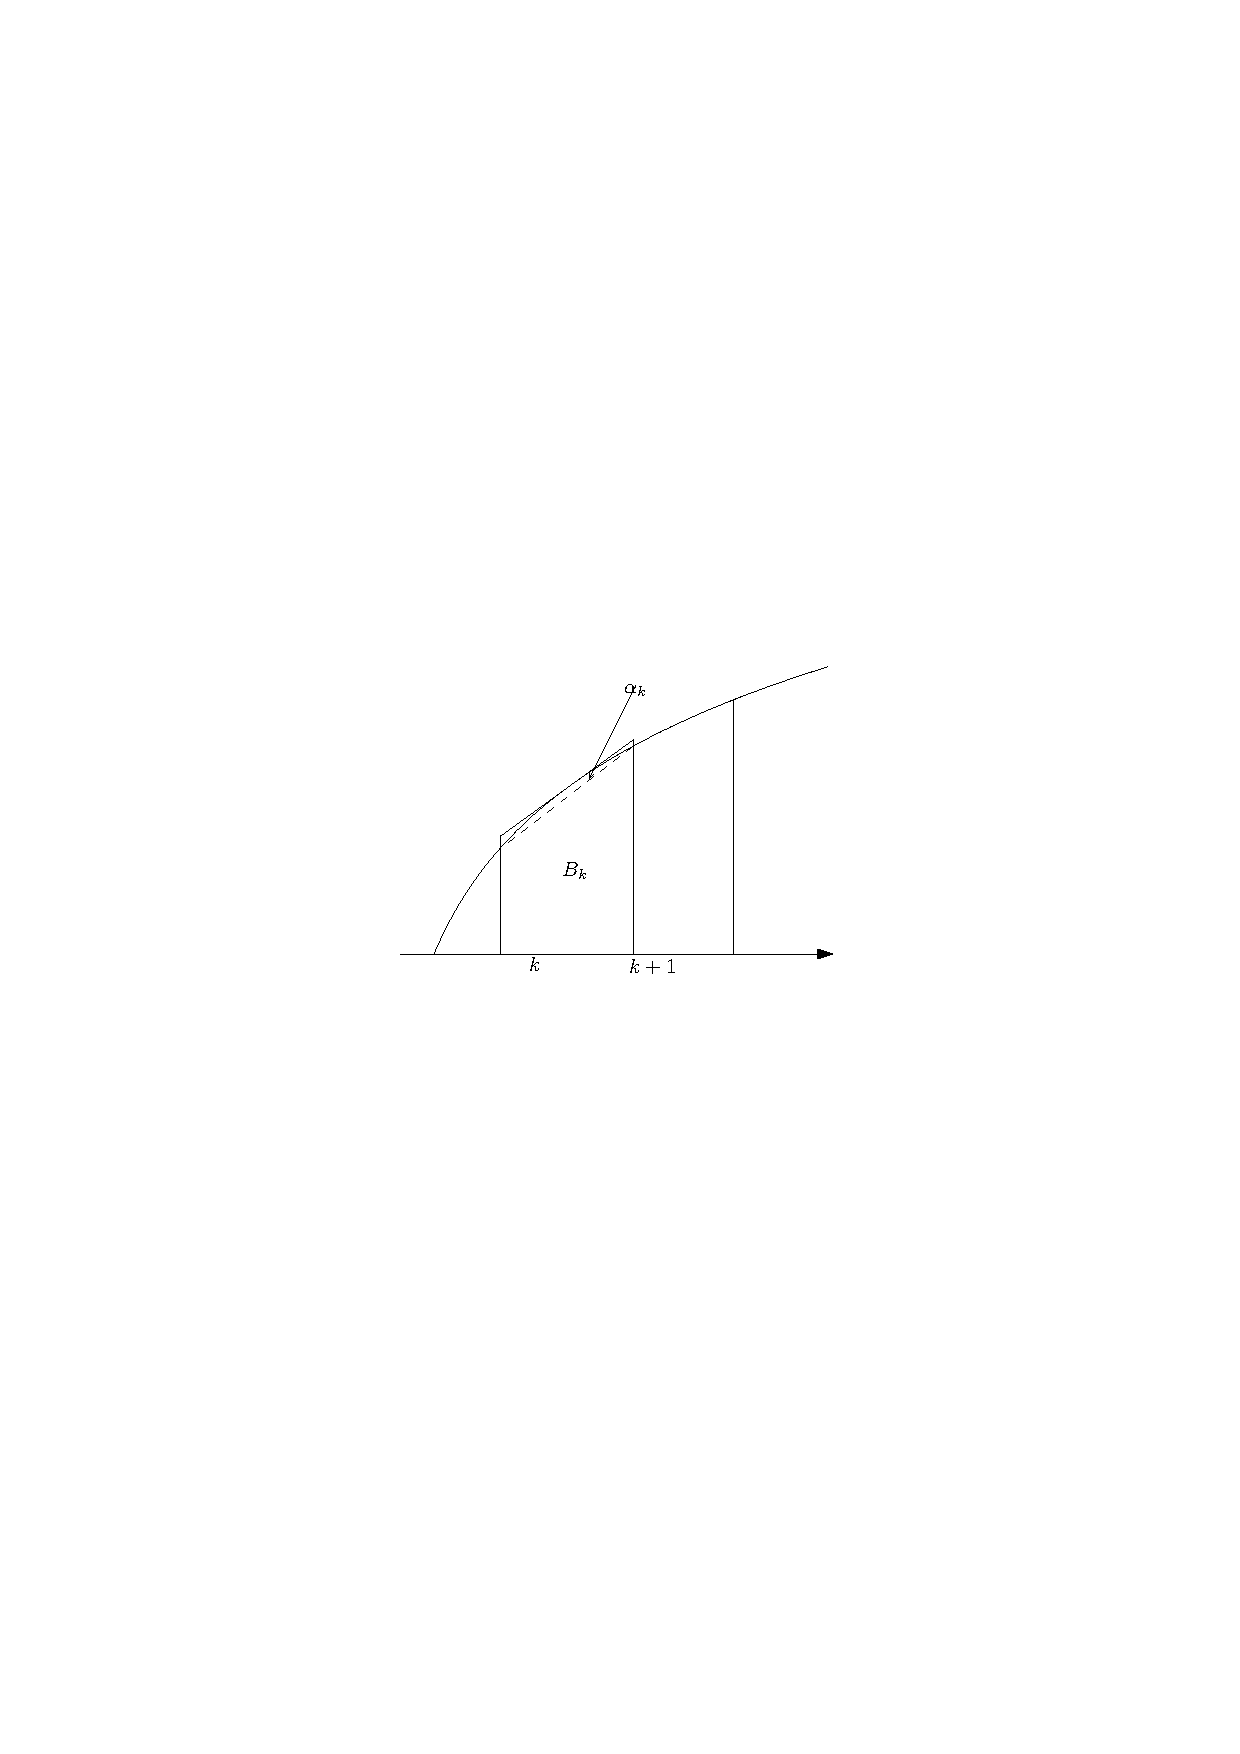
\includegraphics[width=0.5\linewidth]{stirllog}
    \caption{К формуле Стирлинга}
    \label{fig:stirform}
  \end{figure}

  \begin{align*}
    \intertext{Нормальная площадь:}
    A_n &= \int_{1}^{n} \ln x\, dx = \left. ( x \ln x \vphantom{\int} - x)\right|_1^n = n \ln n - n + 1 \\
    \intertext{Приближение:} 
    B_n &= \sum_{k=1}^{n} \left( \frac{\ln(k+1) + \ln(k)}{2} \right) = \ln n! - \frac{1}{2} \ln n \\
    \intertext{Кусочки можно оценить сверху маленькими трапециями, касание там в центре промежутка:} 
    \alpha_k &= \int_k^{k+1} \ln x \, dx - \frac{1}{2} (\ln k + \ln (k+1)) 
    < \ln \left( k + \frac{1}{2} \right) - \frac{1}{2} \big(\ln k + \ln(k+1)\big) \\
    &= \frac{1}{2}\left( \ln\left(1 + \frac{1}{2k}\right) - \ln\left(1+\frac{1}{2k+1}\right) \right)
  \end{align*}
  А тогда $\sum \alpha_k$~--- ряд Лейбница, и 
  \[
    \sum \alpha_k \in \left[0;\frac{1}{2}\ln\lfrac{3}{2}\right], 
    \quad \frac{1}{2} \ln \left( 1 + \frac{1}{2n} \right)  > r_n > 0.
  \]
  Остаток положительный, так как первый член остатка ряда положителен.
  Дальше много преобразований...
  \begin{align*}
    n \ln n - n + 1  - \ln n! + \frac{1}{2} \ln n &= \alpha - r_n \Leftrightarrow \\
    \ln n! &= \left( n+\frac{1}{2} \right) \ln n - n + (1 - \alpha) - r_n 
  \end{align*}
  Теперь разберёмся с остатком
  \[
    e^{r_n} < e^{\frac{1}{2} \ln \left( 1+ \frac{1}{2n} \right)} = \sqrt{1 + \frac{1}{2n}} < 1 + \frac{1}{4n}
  \]
  Таким образом,
  \[
    e^{r_n} = \left( 1 + \frac{\theta}{4n} \right), \;\; \theta\in (0;1)
  \]
  если теперь ещё заменить $c = e^{1-\alpha}$, то получится формула~\ref{thrm:stirform}.
\end{ittproof}
\begin{rem}
  Если приближать не трапециями, а параболами, то можно получить и третью. 
\end{rem}
\begin{thrm}
  Константа $c$ в формуле Стирлинга равна $\sqrt{2\pi}$
\end{thrm}
\begin{ittproof}
  Формулой Валлиса(\ref{thrm:wallisf}) пробьётся.
\end{ittproof}

%<+welcome-to-endofsyn+>
\end{document}
